%!TEX root = ../../Main.tex
\graphicspath{{Chapters/System/}}
%-------------------------------------------------------------------------------


\section{System beskrivelse}
I dette afsnit dannes et overblik over systemets blokke og de interne fobindelser. Derudover gives der et overblik over funktionerne som er implementeret i projektet. 
På figur \ref{fig:Bdd} ses et overordnet Bdd for projektet, hvor de interne forbindelser forklares på figur \ref{fig:Ibd}. 

\begin{figure}[H]
	\centering
	\includegraphics[width = 500 pt]{Img/Bdd.png}
	\caption{Bdd af BA-TA}
	\label{fig:Bdd}
\end{figure}

\textbf{***Skal vi nøjes med et mere simpelt BDD hvor der eksempelvis ikke står noger til Arduinoen og de andre?}

\subsection{Blokbeskrivelse BA-TA}
I det følgende vil komme en beskrivelse af de enkelte blokke i BA-TA og deres interne funktionalitet.
\newline
\newline
\textbf{Arduino} \\*
Arduino'en, mega2560, initialiserer og styrer alt funktionaliteten som indgår i systemet. Arduino blokken står for at initialisere  Touch Display, Touch Controller og Display Controller, som bruges til at kunne modtage signaler fra Touch-delen, samt at sende signaler til Display'et og dermed få repræsenteret noget til brugeren. Yderligere bruges Arduinoen til at kommunikkere med Bluetooth-blokken.
\newline
\newline
\textbf{Touch Controller} \\*
Touch Controller står for at modtage værdier fra Touch Display, samt at sende den modtagede værdi videre til Arduino'en. 
\newline
\newline
\textbf{Display Controller} \\*
Display Controller modtager værdier fra Arduino'en og sende sende værdien videre til Touch Display. \newline
\newline
\textbf{Bluetooth} \\*
Bluetooth modul, HC-05, som kommunikkerer med Arduino'en vha. AT-kommandoer.
\newline
\newline
\textbf{Touch Display} \\*
Touch Display fungerer som brugergrænseflade og er dermed måden brugeren kan interagere med systemet. 
\subsection{Internal Block Diagram for BA-TA}
På figur \ref{fig:Ibd} ses et overordnet IBD over selve systemet, som er bygget på Bdd'et. 
\begin{figure}[H]
	\centering
	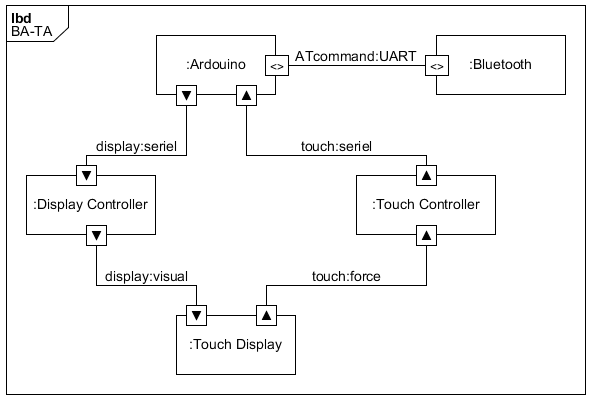
\includegraphics[width = 300 pt]{Img/Ibd.png}
	\caption{Ibd af BA-TA}
	\label{fig:Ibd}
\end{figure}

\subsection{Entity Relationship Diagram for BA-TA}
Herefter gives et overblik på figur \ref{fig:Entity} over koden til driverne som er skrevet til dette projekt.
\textbf{*** Skal opdateres når vi er færdige med alt kode}

\begin{figure}[H]
	\centering
	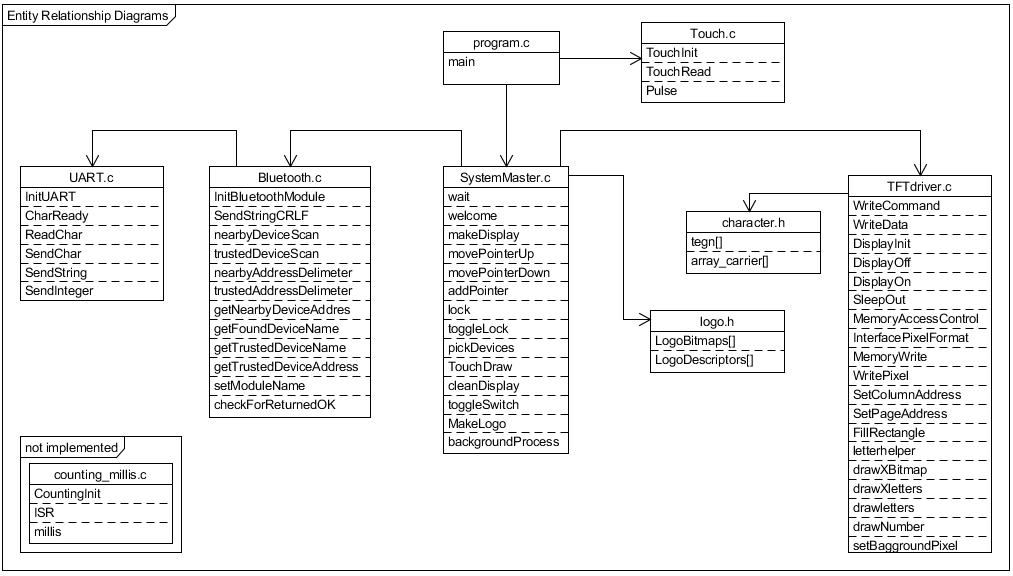
\includegraphics[width = 300 pt]{Img/Entity.png}
	\caption{Entity Relationship Diagrams}
	\label{fig:Entity}
\end{figure}

